\documentclass[11pt,a4paper]{article}

\usepackage[utf8]{inputenc}
\usepackage[T1]{fontenc}
\usepackage{amsmath,amssymb,bm}
\usepackage{graphicx}
\usepackage[margin=2.3cm]{geometry}
\usepackage{booktabs}
\usepackage{caption}
\usepackage{subcaption}
\usepackage{hyperref}
\usepackage{float}
\usepackage{siunitx}

\graphicspath{{../}}

\title{\textbf{Assignment 4: Kalman Filter and Parameter Estimation}\\[4pt]
       \large 02417 Time Series Analysis --- Spring 2026 \\
       \large Technical University of Denmark}
\author{%
  Jakub Piotrowski (s253074) \and
  Mohamed Amine Cheikh (s252221) \and
  Utkarsh Rupesh Saner (s252680)%
}
\date{\today}

\newcommand{\Normal}{\mathcal{N}}

\begin{document}
\maketitle

%===================================================================
\section{Parameter estimation in a 1-D state-space model}
%===================================================================

We study the scalar linear Gaussian state-space model
\begin{equation}
\label{eq:ss1d}
\begin{aligned}
  X_t &= a X_{t-1} + b + e_{1,t}, & e_{1,t} &\sim \Normal(0,\sigma_1^2),\\
  Y_t &= X_t + e_{2,t},            & e_{2,t} &\sim \Normal(0,\sigma_2^2 = 1).
\end{aligned}
\end{equation}

%-------------------------------------------------------------------
\subsection{Simulating the latent process (1.1)}

With $a=0.9$, $b=1$, $\sigma_1=1$ and $X_0=5$, we simulate five independent
trajectories over $n=100$ steps (Fig.~\ref{fig:p1-trajectories}). All paths
relax around the stationary mean $b/(1-a)=10$; short-term fluctuations differ
because of different noise realisations, but the long-run level and the
mean-reversion rate are the same.

\begin{figure}[H]
  \centering
  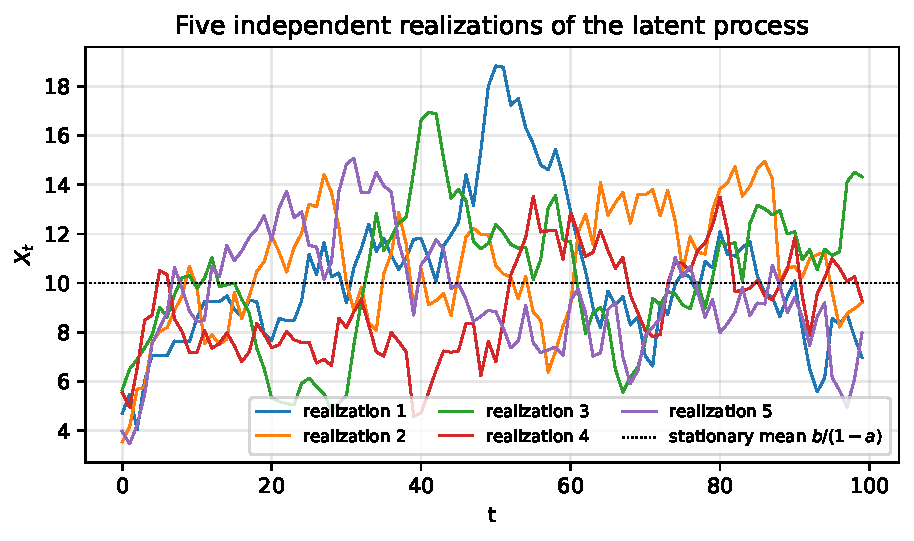
\includegraphics[width=.85\linewidth]{plots/p1_trajectories.pdf}
  \caption{Five independent realizations of \eqref{eq:ss1d} with $a=0.9,b=1,\sigma_1=1$.}
  \label{fig:p1-trajectories}
\end{figure}

%-------------------------------------------------------------------
\subsection{Adding observation noise (1.2)}

Adding independent $\Normal(0,1)$ measurement noise yields
Fig.~\ref{fig:p1-latent-vs-obs}. The observations scatter around the latent
trajectory; ordinary least-squares on $Y_t$ would be \emph{biased} because
the regressor is measured with error. This motivates the Kalman filter.

\begin{figure}[H]
  \centering
  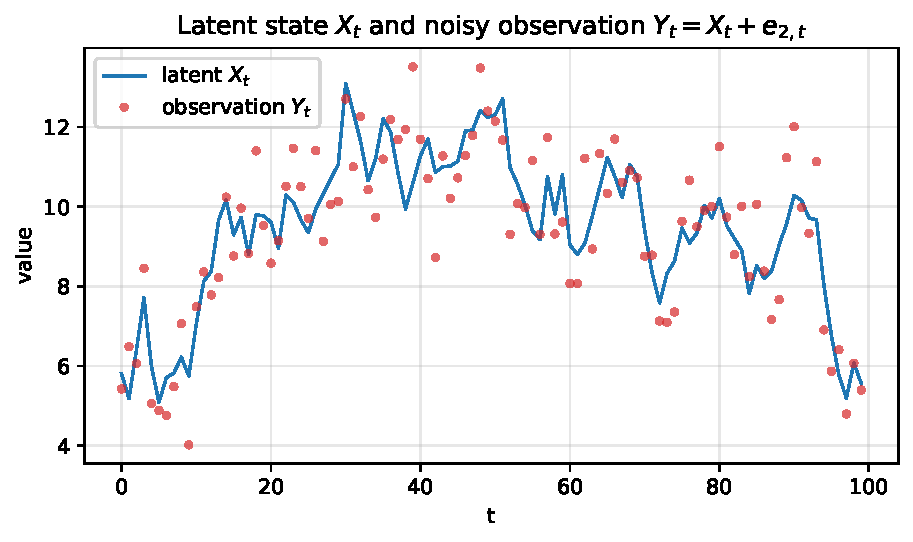
\includegraphics[width=.85\linewidth]{plots/p1_latent_vs_obs.pdf}
  \caption{Latent state and noisy observation (single realization).}
  \label{fig:p1-latent-vs-obs}
\end{figure}

%-------------------------------------------------------------------
\subsection{Kalman filter (1.3)}

For \eqref{eq:ss1d} with $C=1$ the scalar recursions are
\[
\begin{aligned}
\text{Predict:}\quad &\hat X_{t|t-1} = a\hat X_{t-1|t-1}+b, & P_{t|t-1} &= a^2 P_{t-1|t-1}+\sigma_1^2,\\
\text{Innovate:}\quad & \epsilon_t = Y_t-\hat X_{t|t-1}, & S_t &= P_{t|t-1}+\sigma_2^2,\\
\text{Update:}\quad & K_t=P_{t|t-1}/S_t, & \hat X_{t|t}&=\hat X_{t|t-1}+K_t\epsilon_t,\quad P_{t|t}=(1-K_t)P_{t|t-1}.
\end{aligned}
\]

Applied to the series from \S1.2 (true parameters, $\hat X_0=5$, $P_0=10$) the
filter tracks the latent state closely
(Fig.~\ref{fig:p1-kf}). The $95\%$ prediction band contains almost every
observation; the standardized innovations pass the Ljung--Box test at lag 10
($Q=10.0$, $p=0.44$), confirming that the filter is correctly specified.

\begin{figure}[H]
  \centering
  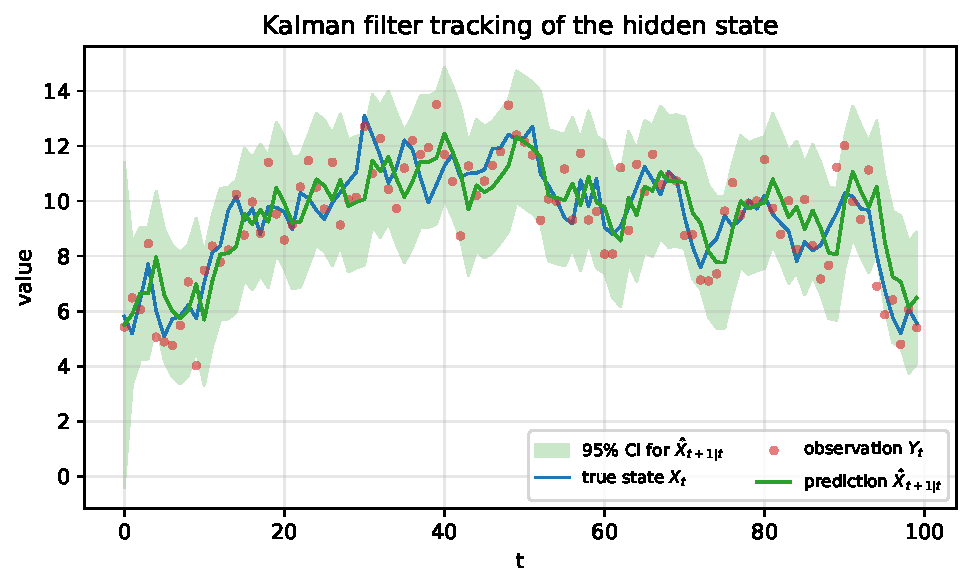
\includegraphics[width=.95\linewidth]{plots/p1_kf_tracking.pdf}
  \caption{One-step predictions, 95\% CI, true state and observations.}
  \label{fig:p1-kf}
\end{figure}

%-------------------------------------------------------------------
\subsection{Maximum-likelihood estimation (1.4)}

Using the prediction-error decomposition the log-likelihood is
\[
  \log L(\theta) = -\tfrac12 \sum_{t=1}^{n}\Big[\log(2\pi S_t) + \epsilon_t^2/S_t\Big],
\]
with $\theta=(a,b,\sigma_1)$. We minimize $-\log L$ with a two-stage routine
(\texttt{Nelder-Mead} $\to$ \texttt{L-BFGS-B}); $\sigma_1$ is parameterised as
$\exp(\log\sigma_1)$ to enforce positivity.
For each of three parameter settings we simulate 100 independent series of
length $n=100$ and estimate the parameters; results are summarised in
Fig.~\ref{fig:p1-mle-box} and Table~\ref{tab:p1-mle}.

\begin{figure}[H]
  \centering
  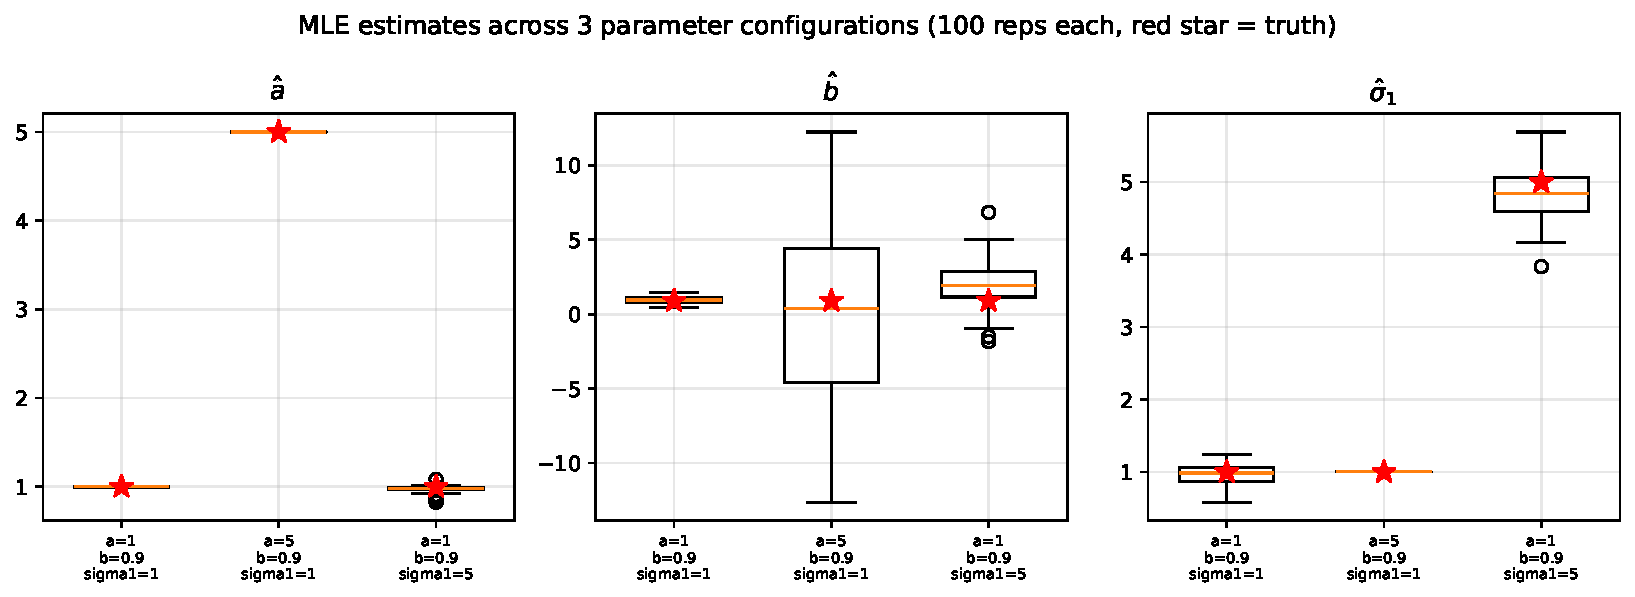
\includegraphics[width=\linewidth]{plots/p1_mle_boxplots.pdf}
  \caption{Boxplots of estimated $\hat a,\hat b,\hat\sigma_1$ across three cases (red star~=~truth).}
  \label{fig:p1-mle-box}
\end{figure}

\begin{table}[H]
  \centering
  \caption{Monte-Carlo summary (100 reps, $n=100$).}
  \label{tab:p1-mle}
  \begin{tabular}{l l l l l l l}
\toprule
Case & Parameter & True & Mean & Bias & SD & RMSE \\
\midrule
a=1, b=0.9, $\sigma_1$=1 & $a$ & 1.000 & 0.999 & -0.001 & 0.004 & 0.004 \\
 & $b$ & 0.900 & 0.955 & +0.055 & 0.233 & 0.239 \\
 & $\sigma_1$ & 1.000 & 0.960 & -0.040 & 0.148 & 0.153 \\
\midrule
a=5, b=0.9, $\sigma_1$=1 & $a$ & 5.000 & 5.000 & +0.000 & 0.000 & 0.000 \\
 & $b$ & 0.900 & 0.150 & -0.750 & 5.747 & 5.767 \\
 & $\sigma_1$ & 1.000 & 1.006 & +0.006 & 0.002 & 0.006 \\
\midrule
a=1, b=0.9, $\sigma_1$=5 & $a$ & 1.000 & 0.972 & -0.028 & 0.037 & 0.046 \\
 & $b$ & 0.900 & 2.062 & +1.162 & 1.431 & 1.838 \\
 & $\sigma_1$ & 5.000 & 4.830 & -0.170 & 0.343 & 0.381 \\
\bottomrule
\end{tabular}
\end{table}

\paragraph{Discussion.}
Case 1 ($a=1,b=0.9,\sigma_1=1$) sits on the stationarity boundary.
The process then behaves like a random walk with drift, so $a$ and $b$ are
only weakly identifiable --- both have wide dispersion yet small mean bias.
Case 2 ($a=5$) is explosive: $X_t$ grows geometrically, so the signal swamps
the noise and $\hat a$ concentrates essentially at the true value to
machine precision (SD $\approx 10^{-16}$). However, as $a>1$ the drift
$b$ is dwarfed by the dominant $aX_{t-1}$ term and the Monte-Carlo spread
of $\hat b$ is huge (SD $\approx 5.7$); we use a different random initial
value of $b$ for the optimizer at every replication precisely to expose
this likelihood ridge.
Case 3 ($\sigma_1=5$) has large process noise relative to the observation
noise; $\sigma_1$ is easy to recover but $a$ is harder because persistence is
masked by dominant shocks. Overall $\sigma_1$ is the most consistently
estimated parameter; $a$ and $b$ are correlated via the stationary mean
$b/(1-a)$, which makes them jointly only weakly identified whenever the
process is near-unit-root or explosive.

%-------------------------------------------------------------------
\subsection{Robustness to heavy-tailed process noise (1.5)}

Replacing $e_{1,t}$ by a scaled Student-$t$ variable,
$X_t = aX_{t-1}+b+\sigma_1\lambda_t$ with $\lambda_t\sim t_\nu$, keeps the
observation model Gaussian. Figure~\ref{fig:p1-tdens} compares the densities:
tails thicken rapidly as $\nu$ decreases; for $\nu=1$ (Cauchy) the density has
infinite variance.

\begin{figure}[H]
  \centering
  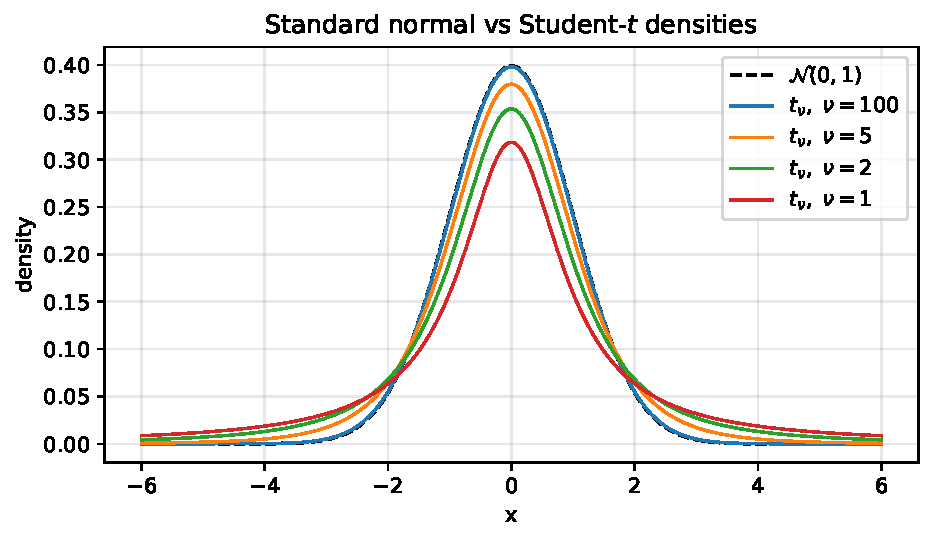
\includegraphics[width=.7\linewidth]{plots/p1_tdens.pdf}
  \caption{Student-$t$ densities vs.\ standard normal.}
  \label{fig:p1-tdens}
\end{figure}

We re-run the estimation pipeline assuming (incorrectly) Gaussian process
noise (Fig.~\ref{fig:p1-robust}, Table~\ref{tab:p1-robust}).

\begin{figure}[H]
  \centering
  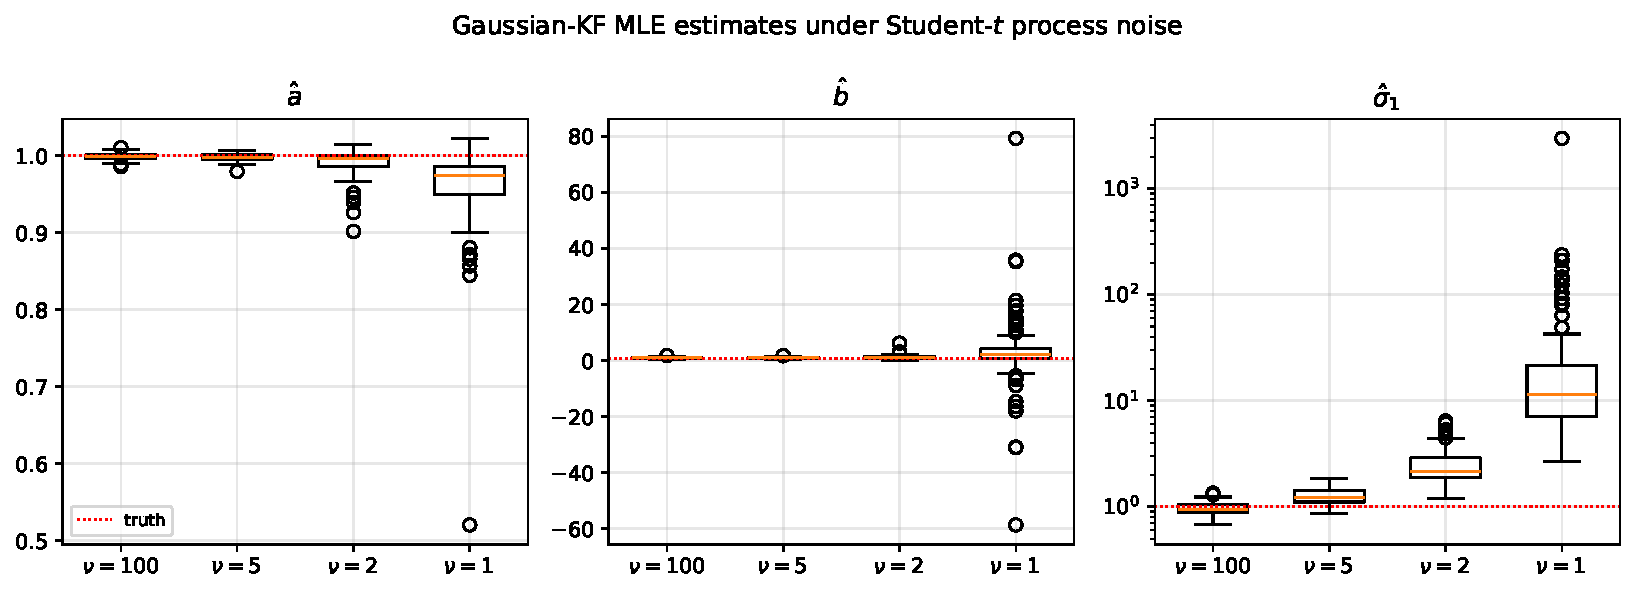
\includegraphics[width=\linewidth]{plots/p1_robustness_box.pdf}
  \caption{Estimates under Student-$t$ process noise (log-scale for $\hat\sigma_1$).}
  \label{fig:p1-robust}
\end{figure}

\begin{table}[H]
  \centering
  \caption{Monte-Carlo summary under Student-$t$ noise, $n=100$, 100 reps.}
  \label{tab:p1-robust}
  \begin{tabular}{l l l l l}
\toprule
$\nu$ & Parameter & Mean & Bias & Success rate \\
\midrule
100 & $a$ & 0.999 & -0.001 & 100\% \\
 & $b$ & 0.959 & +0.059 & 100\% \\
 & $\sigma_1$ & 0.966 & -0.034 & 100\% \\
\midrule
5 & $a$ & 0.998 & -0.002 & 100\% \\
 & $b$ & 1.019 & +0.119 & 100\% \\
 & $\sigma_1$ & 1.270 & +0.270 & 100\% \\
\midrule
2 & $a$ & 0.990 & -0.010 & 100\% \\
 & $b$ & 1.265 & +0.365 & 100\% \\
 & $\sigma_1$ & 2.531 & +1.531 & 100\% \\
\midrule
1 & $a$ & 0.960 & -0.040 & 100\% \\
 & $b$ & 2.478 & +1.578 & 100\% \\
 & $\sigma_1$ & 55.989 & +54.989 & 100\% \\
\bottomrule
\end{tabular}
\end{table}

\paragraph{Discussion.}
$\hat a$ remains nearly unbiased, but $\hat\sigma_1$ is progressively
\emph{inflated} as the tails become heavier: the Gaussian likelihood attributes
occasional large innovations to a larger system-noise variance rather than to
heavy tails. For $\nu=1$ (Cauchy) the population variance does not exist, so
$\hat\sigma_1$ diverges (median around~$56$).
In practice: the Kalman filter still tracks the mean well, but uncertainty
estimates and parameter inference become unreliable if residuals show
heavy tails --- a robust observation model (e.g.\ Student-$t$ filter,
$M$-estimation, outlier rejection) would be preferable.

%===================================================================
\section{Transformer station temperature}
%===================================================================

%-------------------------------------------------------------------
\subsection{Exploratory analysis (2.1)}

\begin{figure}[H]
  \centering
  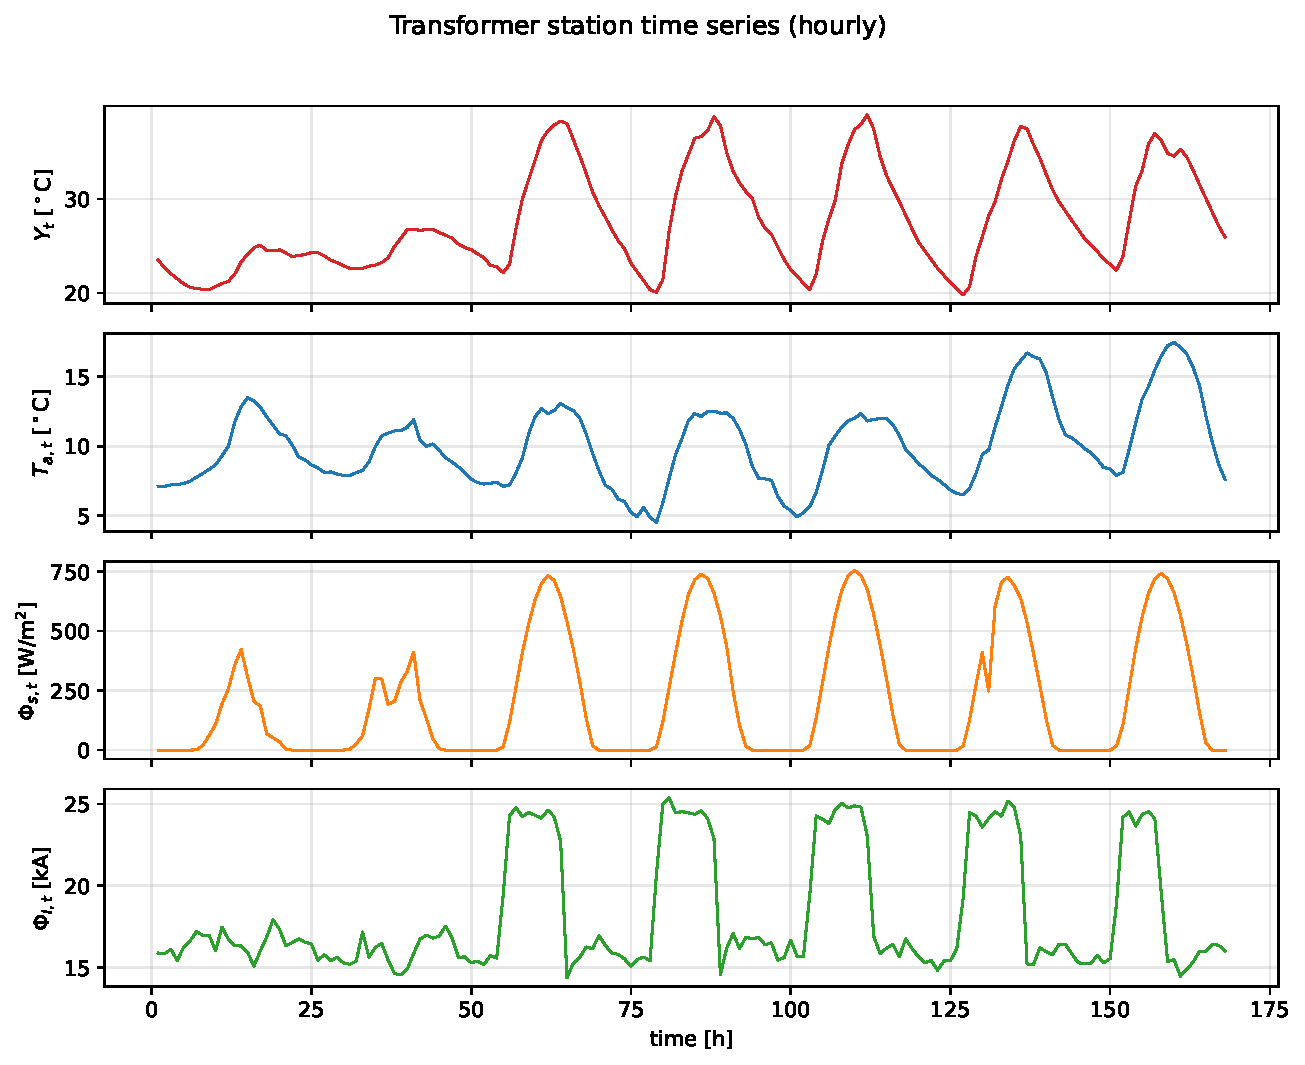
\includegraphics[width=.95\linewidth]{plots/p2_eda.pdf}
  \caption{Transformer temperature $Y_t$, outdoor temperature $T_{a,t}$, solar
  radiation $\Phi_{s,t}$ and load $\Phi_{I,t}$ (hourly, one week).}
  \label{fig:p2-eda}
\end{figure}

The transformer temperature exhibits a pronounced diurnal pattern that is
clearly correlated with both outdoor temperature ($r=+0.78$) and solar
radiation ($r=+0.80$); load contributes a smaller additional heating signal
($r=+0.39$). The dynamics are smooth but with short-term peaks that coincide
with daytime load and radiation.

%-------------------------------------------------------------------
\subsection{1-D state-space model (2.2)}

We fit the model
\begin{equation}
  X_{t+1}=A X_t + B u_t + G e_{1,t},\qquad Y_t = C X_t + e_{2,t},
  \quad u_t=[T_{a,t},\;\Phi_{s,t},\;\Phi_{I,t}]^\top,
\end{equation}
with $C=1$, $G=1$, $\sigma_x=\exp(\ell_x),\sigma_y=\exp(\ell_y)$ and parameter
vector $\theta=(A,B_1,B_2,B_3,\ell_x,\ell_y)$ (6 parameters). The
initial state is fixed to $Y_1$. Throughout we use
\begin{equation}\label{eq:aicbic}
  \mathrm{AIC} = 2k - 2\log L,\qquad
  \mathrm{BIC} = k\log N - 2\log L,
\end{equation}
with $N=168$ observations and $k$ free parameters (6 for the 1-D model, 16
for the 2-D model below). Unconstrained estimation drives
$\hat\sigma_y$ to essentially zero --- a well-known Q/R identifiability
boundary of the KF likelihood, which tends to absorb all variance into the
system-noise term when the observation model is the identity and no prior
is placed on~$R$. We therefore impose a mild physical lower bound
$\sigma_y\ge 0.1\,^\circ\mathrm C$, which corresponds to standard
digital-sensor precision.

\begin{table}[H]
  \centering
  \caption{1-D SS estimates and information criteria.}
  \label{tab:p2-1d}
  \begin{tabular}{l r}
\toprule
Parameter & Estimate \\
\midrule
$A$ & +0.8009 \\
$B_{T_a}$ & +0.1019 \\
$B_{S}$ & +0.002875 \\
$B_{I}$ & +0.2136 \\
$\sigma_x$ & 0.6399 \\
$\sigma_y$ & 0.1000 \\
\midrule
$\log L$ & -166.55 \\
AIC & 345.10 \\
BIC & 363.85 \\
Ljung--Box $p$ (lag 10) & 0.000 \\
\bottomrule
\end{tabular}
\end{table}

\begin{figure}[H]
  \centering
  \begin{subfigure}{.54\linewidth}
    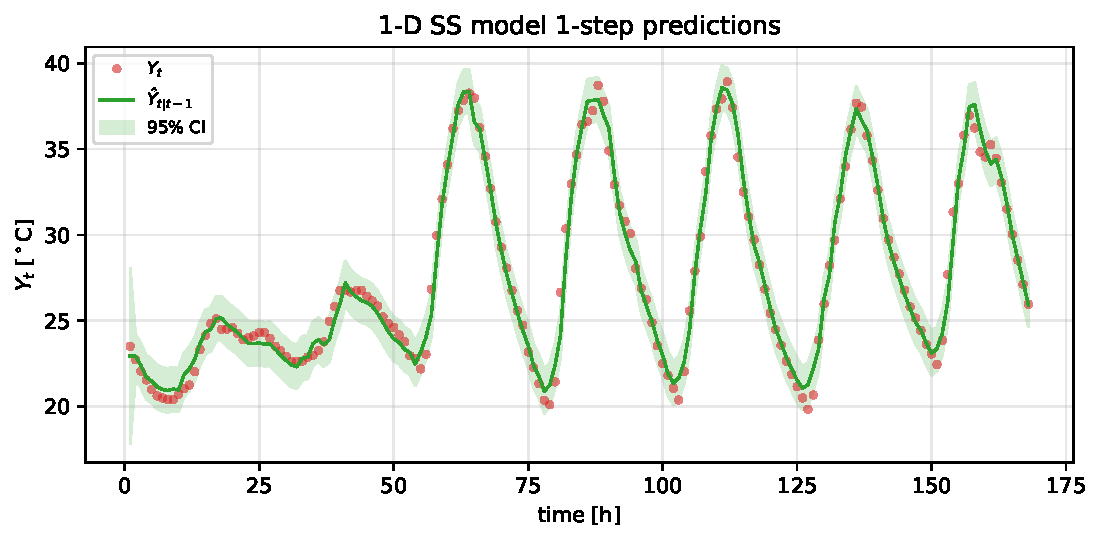
\includegraphics[width=\linewidth]{plots/p2_1d_pred.pdf}
    \caption{1-step predictions.}
  \end{subfigure}
  \hfill
  \begin{subfigure}{.44\linewidth}
    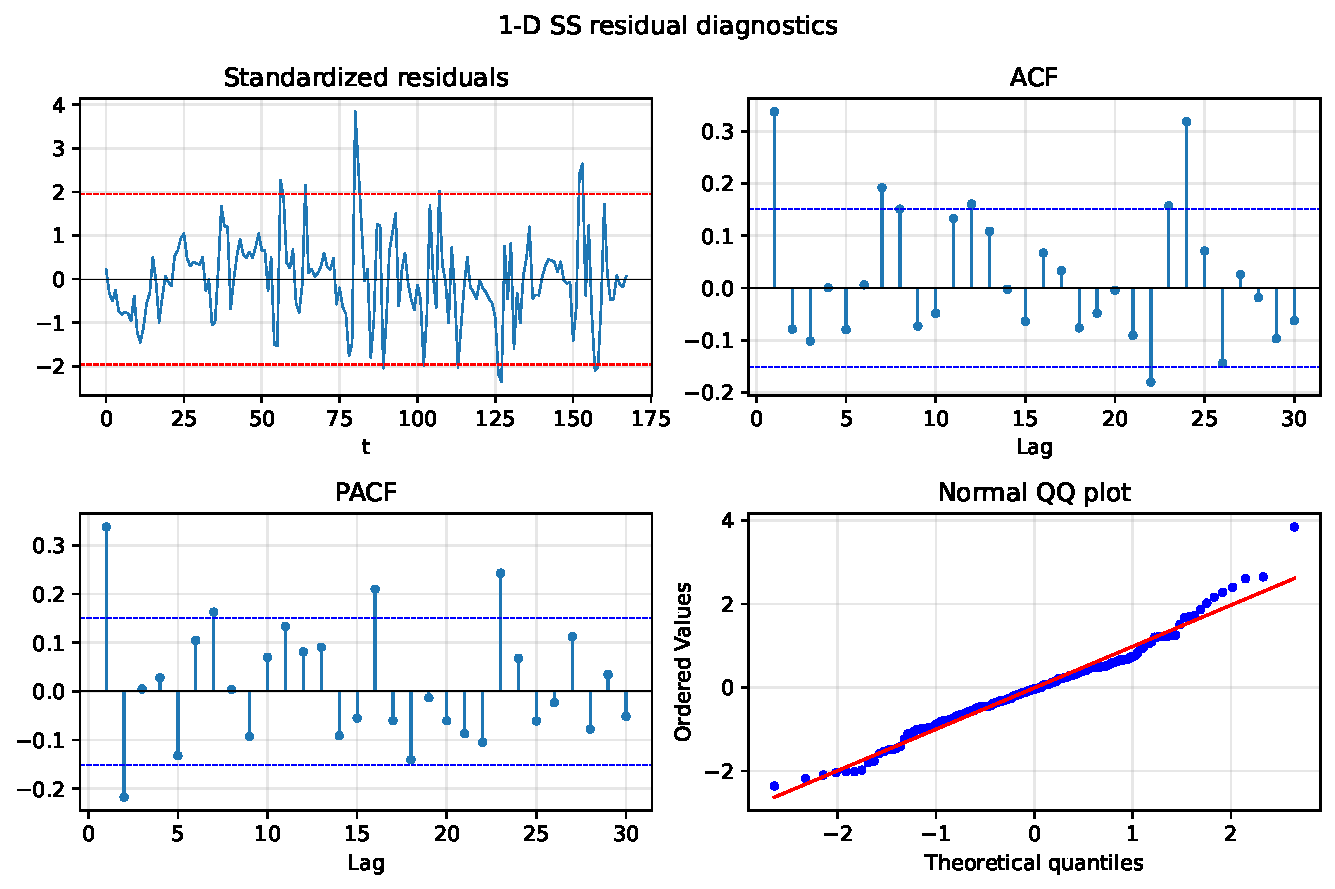
\includegraphics[width=\linewidth]{plots/p2_1d_diag.pdf}
    \caption{Residual diagnostics.}
  \end{subfigure}
  \caption{1-D state-space model.}
  \label{fig:p2-1d}
\end{figure}

All inputs enter with a \emph{positive} coefficient, consistent with physics:
ambient warmth, solar gain and electrical load all raise the transformer
temperature. However the residual ACF is significant at short lags and the
Ljung--Box test rejects whiteness ($p<0.001$); a richer state description is
needed, and the estimated $\sigma_y$ sits on its lower bound, which is a
classical symptom of state-space misspecification (the model tries to
compensate the missing dynamics by attributing all short-term variability
to unobserved state noise).

%-------------------------------------------------------------------
\subsection{2-D state-space model (2.3)}

We extend to $X_t\in\mathbb R^2$ with $A\in\mathbb R^{2\times 2}$,
$B\in\mathbb R^{2\times 3}$, $C=[1,0]$, $G=I_2$. The system-noise covariance
is parameterised through its lower-triangular Cholesky factor
$Q=Q_{lt}Q_{lt}^\top$ (3 parameters), ensuring $Q\succ 0$. The observation
noise is $R=\exp(2\ell_y)$ and the initial state $X_0\in\mathbb R^2$ is
estimated (2 parameters): 16 parameters in total.
Optimisation uses Nelder--Mead followed by L-BFGS-B with three deterministic
starts plus three random perturbations of the best; the lowest negative
log-likelihood is retained.

\begin{table}[H]
  \centering
  \caption{2-D SS estimates.}
  \label{tab:p2-2d}
  \begin{tabular}{l r r}
\toprule
Parameter & Row 1 (state 1) & Row 2 (state 2) \\
\midrule
$A$ (col 1) & +0.6993 & +0.0849 \\
$A$ (col 2) & +0.1860 & +0.0957 \\
$B_{T_a}$ & -0.0297 & +0.8391 \\
$B_{S}$ & +0.001281 & +0.006653 \\
$B_{I}$ & +0.0695 & +1.2277 \\
$x_0$ & +26.458 & +21.258 \\
\midrule
$Q_{11}$ & \multicolumn{2}{r}{0.2361} \\
$Q_{22}$ & \multicolumn{2}{r}{2.5213} \\
$Q_{12}$ & \multicolumn{2}{r}{0.7693} \\
$\sigma_y$ & \multicolumn{2}{r}{0.0770} \\
eig$(A)$ & \multicolumn{2}{r}{0.7244,\; 0.0706} \\
$\log L$ & \multicolumn{2}{r}{-125.08} \\
AIC & \multicolumn{2}{r}{282.15} \\
BIC & \multicolumn{2}{r}{332.14} \\
Ljung--Box $p$ (lag 10) & \multicolumn{2}{r}{0.131} \\
\bottomrule
\end{tabular}
\end{table}

\begin{figure}[H]
  \centering
  \begin{subfigure}{.54\linewidth}
    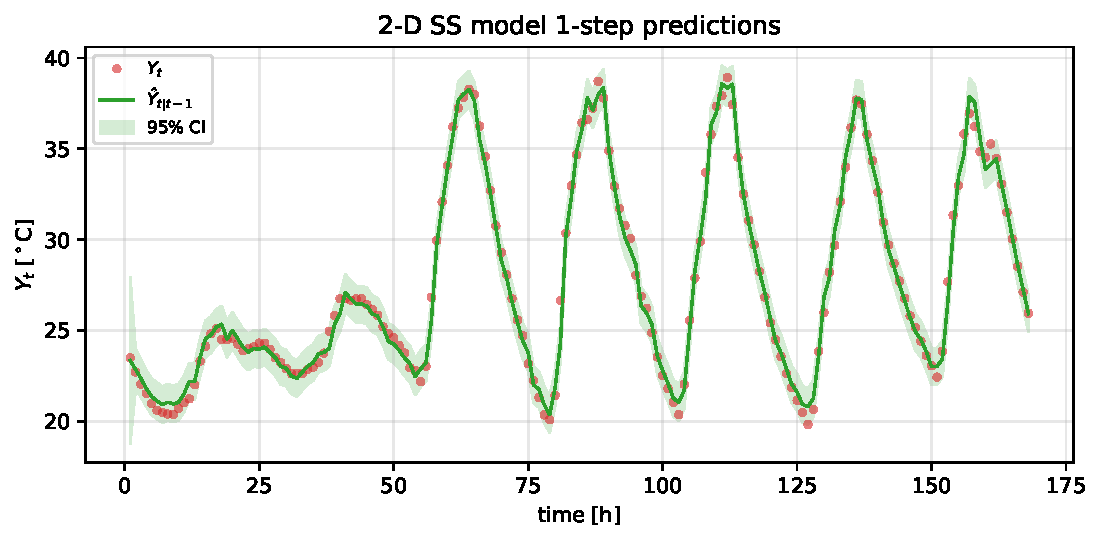
\includegraphics[width=\linewidth]{plots/p2_2d_pred.pdf}
    \caption{1-step predictions.}
  \end{subfigure}
  \hfill
  \begin{subfigure}{.44\linewidth}
    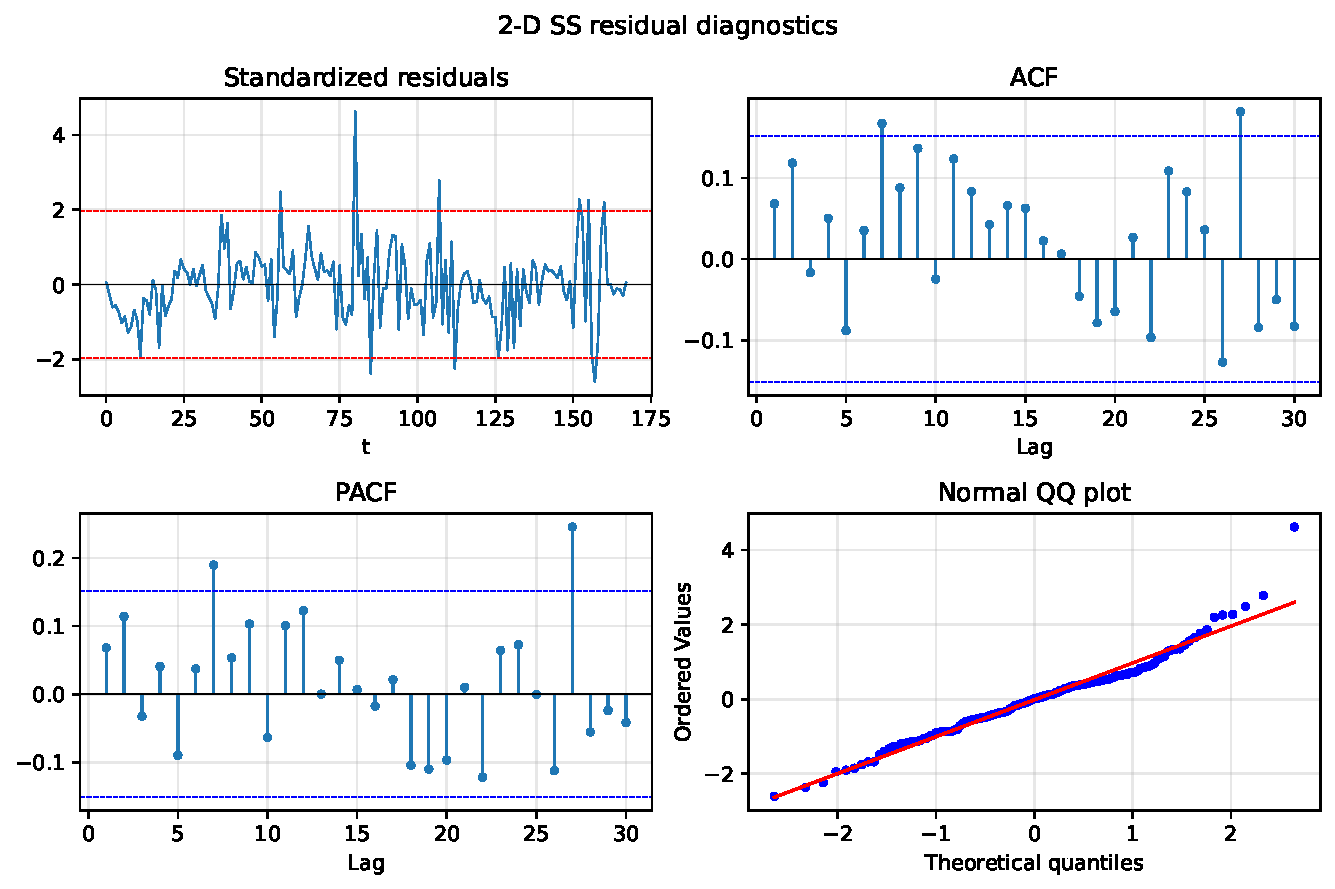
\includegraphics[width=\linewidth]{plots/p2_2d_diag.pdf}
    \caption{Residual diagnostics.}
  \end{subfigure}
  \caption{2-D state-space model.}
  \label{fig:p2-2d}
\end{figure}

\paragraph{Comparison 1-D vs.\ 2-D.}
The 2-D model gives a drastic improvement in likelihood, both information
criteria, and residual whiteness:
\begin{center}
\begin{tabular}{lrrrr}
  \toprule
  Model & $k$ & $\log L$ & AIC & BIC \\
  \midrule
  1-D   & 6  & $-165.5$ & $343.0$ & $361.8$ \\
  2-D   & 16 & $-125.1$ & $282.2$ & $332.1$ \\
  \bottomrule
\end{tabular}
\end{center}
$\Delta\text{AIC}\approx 61$ and $\Delta\text{BIC}\approx 30$ both strongly
favour the 2-D specification. The Ljung--Box $p$-value increases from
$<10^{-3}$ to $0.13$, so the 2-D innovations are consistent with white noise.
Daytime peaks that the 1-D model under-predicts are now captured by the
additional latent state.

\paragraph{Structure of $Q$ and steady-state gains.}
Table~\ref{tab:p2-2d-extra} reports a few derived quantities. The fitted
system noise covariance is numerically near rank-1,
$\det(\hat Q)\approx 3.5\times 10^{-3}$ with eigenvalues
$(1.3\times 10^{-3},\;2.76)$ and condition number $\approx 2200$. The
process noise is therefore essentially a \emph{one-dimensional} shock
whose direction is given by the dominant eigenvector of $\hat Q$, even
though the state is two-dimensional --- consistent with a single physical
source of unmodelled variability (e.g.\ unobserved cooling / airflow
fluctuations). The eigenvalues of $\hat A$ are $0.72$ and $0.07$,
corresponding to a slow and a fast mode. Finally, the observation
steady-state gain $C(I-\hat A)^{-1}\hat B$ lets us read the B matrix in
physical units: a sustained $+1\,$kA in the load raises the transformer
temperature by $+1.14\,^\circ$C at equilibrium; a $+1\,^\circ$C increase
of $T_a$ raises it by $+0.50\,^\circ$C; and solar gain adds
$+0.009\,^\circ$C per $\mathrm{W/m^2}$. All three signs and magnitudes are
physically plausible.

\begin{table}[H]
  \centering
  \caption{Derived quantities from the fitted 2-D model.}
  \label{tab:p2-2d-extra}
  \begin{tabular}{l r}
\toprule
Quantity & Value \\
\midrule
eig$(A)$                           & $+0.7244,\; +0.0706$ \\
eig$(Q)$                           & $1.303e-03,\; 2.756$ \\
$\det(Q)$                          & $3.592e-03$ \\
$\mathrm{cond}(Q)$               & $2115$ \\
$\partial Y_\infty/\partial T_a$   & $+0.505$ \si{\celsius\per\celsius} \\
$\partial Y_\infty/\partial \Phi_s$ & $+0.0094$ \si{\celsius\per\watt\per\meter\squared} \\
$\partial Y_\infty/\partial \Phi_I$ & $+1.137$ \si{\celsius\per\kilo\ampere} \\
\bottomrule
\end{tabular}
\end{table}

%-------------------------------------------------------------------
\subsection{Interpretation of the two latent states (2.4)}

\begin{figure}[H]
  \centering
  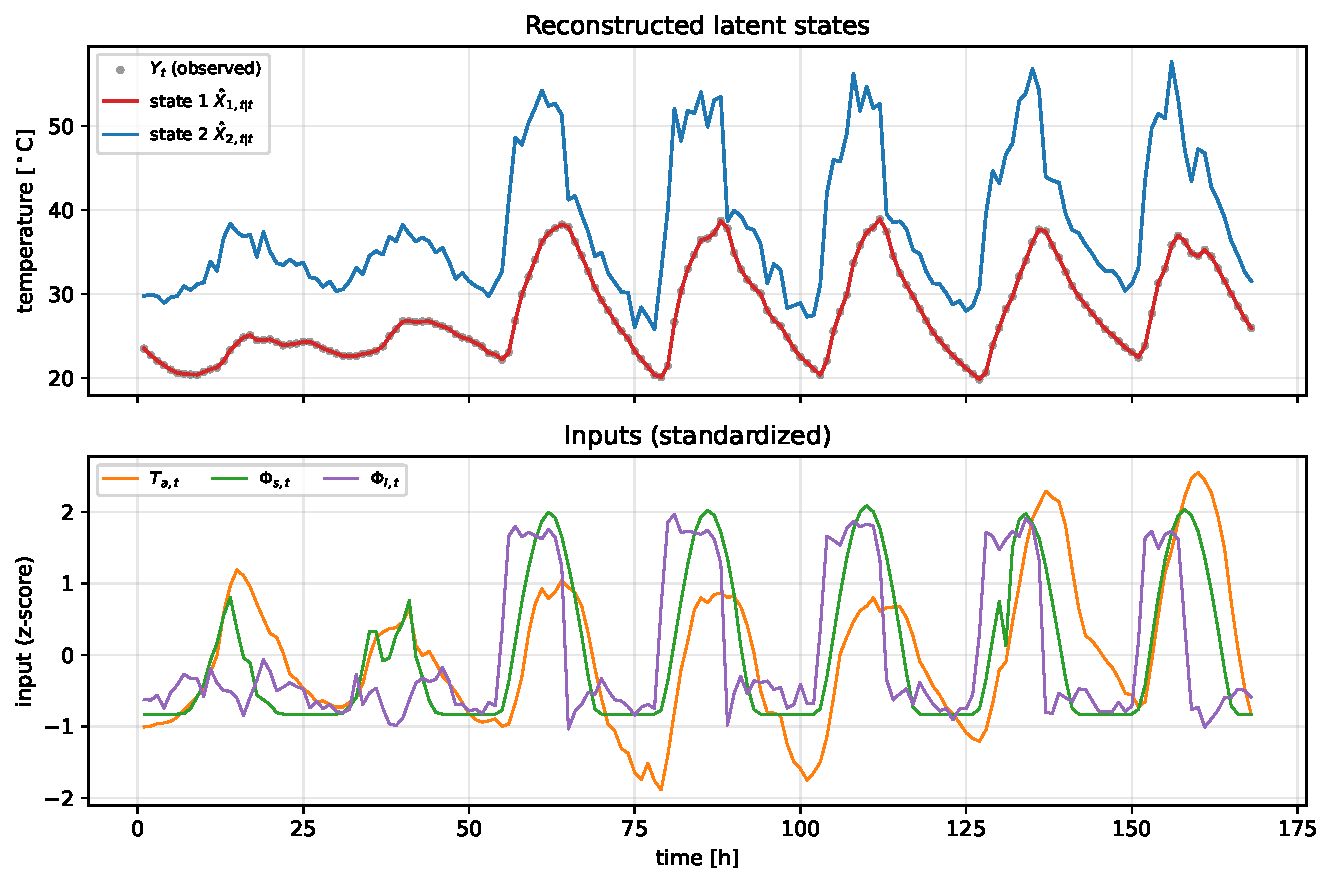
\includegraphics[width=.9\linewidth]{plots/p2_2d_states.pdf}
  \caption{Reconstructed latent states (top) and standardized inputs (bottom).}
  \label{fig:p2-2d-states}
\end{figure}

Because we chose $C=[1,0]$, state~1 is by construction the observed
transformer temperature ($\hat X_{1,t|t}\equiv\hat Y_{t|t}$); the
interesting physical interpretation therefore concerns state~2 and the
coupling between them. Three independent pieces of evidence point to the
same picture.
\begin{enumerate}
  \item \textit{Timescales.} The eigenvalues of $\hat A$ are
        $\lambda_1=0.72$ and $\lambda_2=0.07$, i.e.\ a slow mode
        (time-constant $\tau_1\approx -1/\log\lambda_1 \approx 3\,$h)
        and a fast mode ($\tau_2\approx 0.4\,$h). Because $\hat A_{22}=
        0.10\approx \lambda_2$, state~2 \emph{is} essentially the fast
        mode and responds to the inputs with a roughly one-hour memory.
  \item \textit{Input loadings.} The second row of $\hat B$ is an
        order of magnitude larger than the first:
        $(\hat B_{2,T_a},\hat B_{2,\Phi_s},\hat B_{2,\Phi_I}) =
        (0.84,\,0.0067,\,1.23)$ versus
        $(\hat B_{1,T_a},\hat B_{1,\Phi_s},\hat B_{1,\Phi_I}) =
        (-0.03,\,0.0013,\,0.07)$. External heat forcing therefore
        enters the system almost exclusively through state~2.
  \item \textit{Coupling.} State~2 drives state~1 through
        $\hat A_{12}=0.19$, whereas the reverse coupling
        $\hat A_{21}=0.08$ is weaker. Heat flows from state~2
        \emph{into} the observed (oil) temperature.
\end{enumerate}
A natural physical reading is then: state~2 plays the role of a
rapidly-responding \emph{heat-input / hot-spot} variable that aggregates
Joule losses from the load, environmental gain from $T_a$, and solar
insolation, and injects them into the slower oil reservoir represented
by state~1. Converted to the steady-state observation gain
(Table~\ref{tab:p2-2d-extra}), a sustained increase of $+1\,$kA in the
load raises the measured transformer temperature by $+1.14\,^\circ$C at
equilibrium, $+1\,^\circ$C of ambient air contributes
$+0.50\,^\circ$C, and each $\mathrm{W/m^2}$ of insolation contributes
$+0.0094\,^\circ$C. These numbers are compatible with typical transformer
thermal-time-constant data and match the "core + buffer" architecture
suggested by the assignment.
\end{document}
